\chapter{Interfejs użytkownika}\label{chap:ui}
Do stworzenia interfejsu użytkownika (UI) za wzorce użyliśmy gier “MountAndBlade”, “MountAndBlade2 Bannerlord”, “Warcraft3”, “The Elder Scrolls V: Skyrim”, “Orcs must die”aby umożliwić graczowi jak najprzyjemniejszą rozrywkę oraz wszystkie potrzebne funkcje.

Pierwszy ekran
Wzorowanie: “MountAndBlade”
Jako pierwszy ekran, który widzi gracz przewidujemy grafikę z możliwością wybrania jednej z opcji z menu głównego.

Poruszanie się

Przewidujemy:
górny pasek z najważniejszymi informacjami:surowce, fundusze, czas, kompas
ikony postaci, na które gracz może się przełączyć;
obszar dla komentarzy
pasek życia.

Inspiracja dla górnego paska z najważniejszymi informacjami:surowce, fundusze, czas oraz ikon postaci, na które gracz może się przełączyć:
\begin{figure}[htbp]
    \centering
    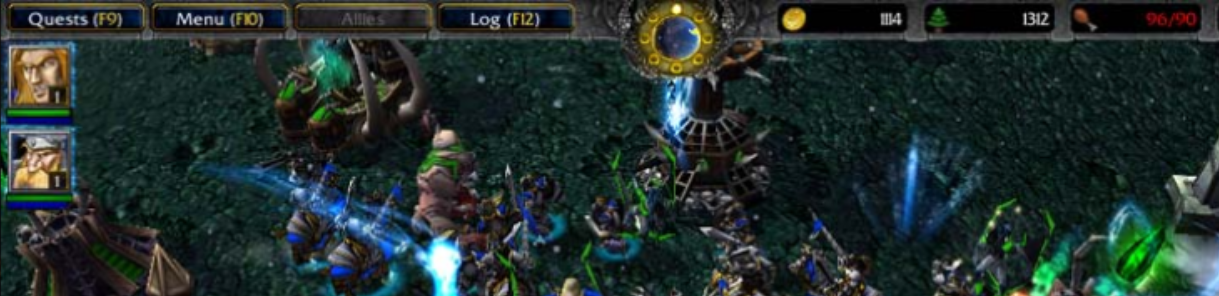
\includegraphics[width=0.9\textwidth]{images/ui/warcraft3.png}
    \caption{źródło: Warcraft 3.}\label{fig:Warcraft3}
\end{figure}

Inspiracja dla kompasu:
\begin{figure}[htbp]
    \centering
    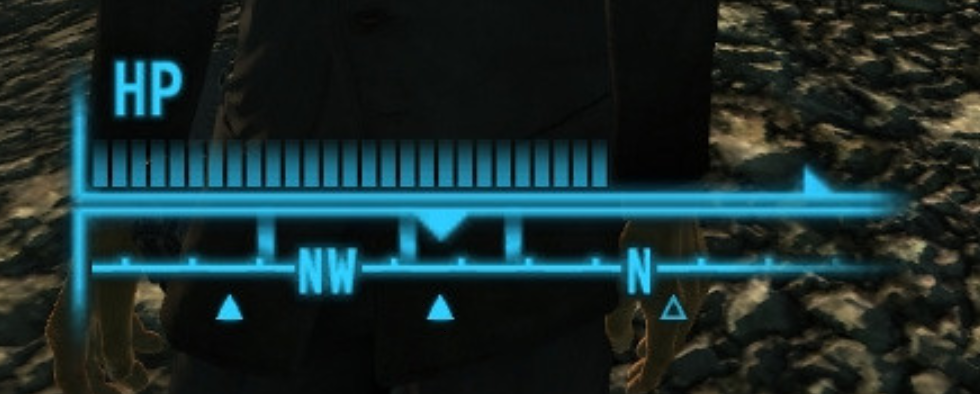
\includegraphics[width=0.9\textwidth]{images/ui/compassSkyrim.png}
    \caption{źródło: Fallout.}\label{fig:Fallout}
\end{figure}

Rozmowa 
\begin{figure}[htbp]
    \centering
    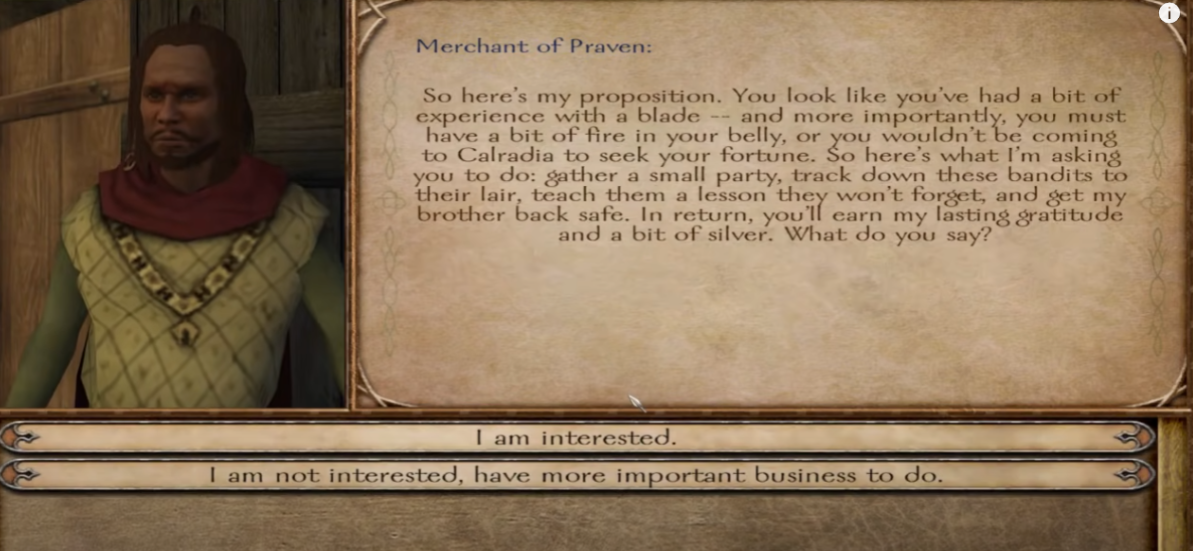
\includegraphics[width=0.9\textwidth]{images/ui/conversationMnB.png}
    \caption{źródło: MountAndBlade.}\label{fig:MountnBlade}
\end{figure}

Walka
Przy walce dostępne materiały zamienią się na pasek pokazujący sumaryczne życie naszej drużyny i drużyny przeciwnej oraz możliwe komendy do wydania.

Inspiracja dla możliwych komend:
\begin{figure}[htbp]
    \centering
    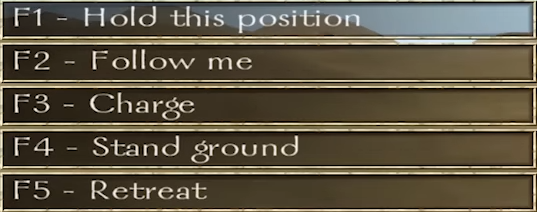
\includegraphics[width=0.9\textwidth]{images/ui/commandsMountBla.png}
    \caption{źródło: MountAndBlade.}\label{fig:MountnBlade}
\end{figure}


Budowa budynków
W tym trybie pokażą nam się dostępne do zbudowania budynki, a po wybraniu pojawią się przed nami. Po zatwierdzeniu budynek zostanie wybudowany.

Inspiracja dla trybu budowania:
\begin{figure}[htbp]
    \centering
    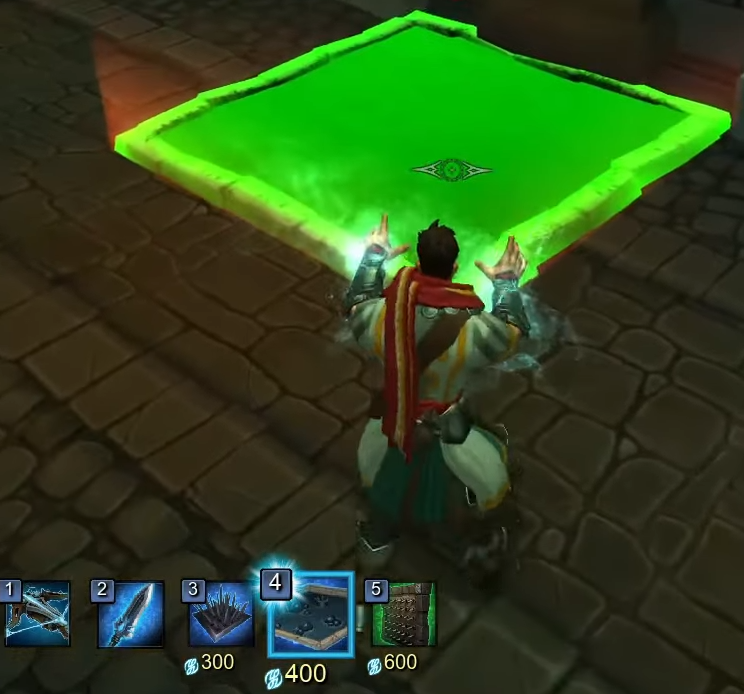
\includegraphics[width=0.9\textwidth]{images/ui/buoildingsOrcs.png}
    \caption{źródło: Orcs must die}\label{fig:Orcs}
\end{figure}

